\chapter{\sffamily Describing the time evolution of probabilities}

{\bfseries\sffamily Concept.} To extend the formalism that we developed in the previous chapter to help us better understand the time evolution of state probabilities. With this knowledge we shall derive popular machine learning methods like Gaussian processes, as well as discussing how some phenomena permit a convenient description via mean field equations or regression of distribution moments. For the mathematically-inclined, this chapter will take a detailed look at how our formalism can be extended to focus on the time evolution of probabilities, with a view to statistical inference later on. For the programmers, all of the relevant software lives in this public Git repository: \href{https://github.com/umbralcalc/learndadex}{https://github.com/umbralcalc/learnadex}.

\section{\sffamily Probabilistic formalism}

Let's start by returning to the formalism that we introduced in the previous chapter. As we discussed at that point; this formalism is appropriate for sampling from nearly every stochastic phenomenon that one can think of. We are going to extend this description to consider what happens to the probability that the state history matrix takes a particular set of values over time.

\begin{figure}[h]
\centering
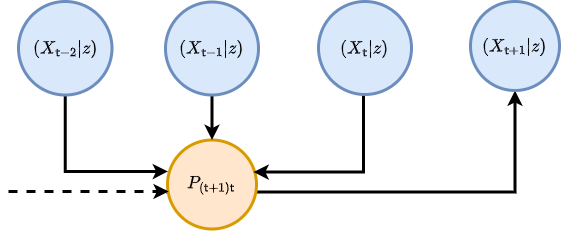
\includegraphics[width=12cm]{images/chapter-2-master-eq-graph.drawio.png}
\caption{Graph representation of Eq.~(\ref{eq:master-x-cont}).}
\label{fig:master-eqn}
\end{figure} 

So, how do we begin? In the first chapter, we defined the general stochastic process with the formula $X^{i}_{{\sf t}+1} = F^{i}_{{\sf t}+1}(X_{0:{\sf t}},z,{\sf t})$. This equation also has an implicit \emph{master equation} associated to it that fully describes the time evolution of the \emph{probability density function} $P_{{\sf t}+1}(X\vert z)$ of $X_{0:{\sf t}+1}=X$ given that the parameters of the process are $z$. This can be written as
%%
\begin{align}
P_{{\sf t}+1}(X\vert z) &= P_{{\sf t}}(X'\vert z) P_{({\sf t}+1){\sf t}}(x\vert X',z) \label{eq:master-x-cont}\,,
\end{align}
%%
where for the time being we are assuming the state space is continuous in each of the matrix elements and $P_{({\sf t}+1){\sf t}}(x\vert X',z)$ is the conditional probability that $X_{{\sf t}+1}=x$ given that $X_{0:{\sf t}}=X'$ at time ${\sf t}$ and the parameters of the process are $z$. To try and understand what Eq.~(\ref{eq:master-x-cont}) is saying, we find it's helpful to think of an iterative relationship between probabilities; each of which is connected by their relative conditional probabilities. We've also illustrated this kind of thinking in Fig.~\ref{fig:master-eqn}.

Consider what happens when we extend the chain of conditional probabilities in Eq.~(\ref{eq:master-x-cont}) back in time by one step. In doing so, we retrieve a joint probability of rows $X_{{\sf t}+1}=x$ and $X_{{\sf t}}=x'$ on the right hand side of the expression 
%%
\begin{align}
P_{{\sf t}+1}(X\vert z) &= P_{{\sf t}-1}(X''\vert z) P_{({\sf t}+1){\sf t}({\sf t}-1)}(x,x'\vert X'',z) \label{eq:master-x-pairwise-joint}\,.
\end{align}
%%
Since Eqs.~(\ref{eq:master-x-cont}) and~(\ref{eq:master-x-pairwise-joint}) are both valid ways to obtain $P_{{\sf t}+1}(X\vert z)$ we can average between them without loss of generality in the original expression, like this
%%
\begin{align}
P_{{\sf t}+1}(X\vert z) &= \frac{1}{2}\big[ P_{{\sf t}}(X'\vert z) P_{({\sf t}+1){\sf t}}(x\vert X',z) + P_{{\sf t}-1}(X''\vert z) P_{({\sf t}+1){\sf t}({\sf t}-1)}(x,x'\vert X'',z) \big]\,.
\end{align}
%%
Following this line of reasoning to its natural conclusion, Eq.~(\ref{eq:master-x-cont}) can hence be generalised to consider all possible joint distributions of rows at different timesteps like this
%%
\begin{align}
P_{{\sf t}+1}(X\vert z) &= \frac{1}{{\sf t}}\sum_{{\sf t}''=0}^{{\sf t}}P_{{\sf t}''}(X''\vert z) P_{({\sf t}+1){\sf t}\dots{\sf t}''}(x,x',\dots \vert X'',z) \label{eq:master-x-cont-sum-gen}\,.
\end{align}
%%

If we wanted to just look at the distribution over the latest row $X_{{\sf t}+1}=x$, we could achieve this through marginalisation over all of the previous matrix rows in Eq.~(\ref{eq:master-x-cont}) like this
%%
\begin{align}
P_{{\sf t}+1}(x\vert z) = \int_{\Omega_{{\sf t}}}{\rm d}X' P_{{\sf t}+1}(X\vert z) &= \int_{\Omega_{{\sf t}}}{\rm d}X' P_{{\sf t}}(X'\vert z) P_{({\sf t}+1){\sf t}}(x\vert X',z) \label{eq:master-x-cont-latest-row} \,.
\end{align}
%%
But what is $\Omega_{\sf t}$? You can think of this as just the domain of possible matrix $X'$ inputs into the integral which will depend on the specific stochastic process we are looking at. 

The symbol ${\rm d}X'$ in Eq.~(\ref{eq:master-x-cont-latest-row}) is our shorthand notation throughout the book for computing the sum of integrals over previous state history matrices which can further be reduced via Eq.~(\ref{eq:master-x-cont-sum-gen}) into a product of sub-domain integrals over each matrix row
%%
\begin{align}
P_{{\sf t}+1}(x\vert z) &= \frac{1}{{\sf t}}\sum_{{\sf t}''=0}^{{\sf t}} \bigg\lbrace \int_{\omega_{{\sf t}'}}{\rm d}^nx'...\int_{\Omega_{{\sf t}''}}{\rm d}X'' \bigg\rbrace \,P_{{\sf t}''}(X''\vert z) P_{({\sf t}+1){\sf t}\dots{\sf t}''}(x,x',... \vert X'',z) \\
&= \frac{1}{{\sf t}}\sum_{{\sf t}''=0}^{{\sf t}} \int_{\Omega_{{\sf t}''}}{\rm d}X'' P_{{\sf t}''}(X''\vert z) P_{({\sf t}+1){\sf t}''}(x \vert X'',z) \label{eq:master-x-cont-latest-row-gen} \,,
\end{align}
%%
where each row measure is a Cartesian product of $n$ elements (a Lebesgue measure), i.e.,
%%
\begin{align}
{\rm d}^nx = \prod_{i=0}^n{\rm d}x^i \,,
\end{align}
%%
and lowercase $x, x', \dots$ values will always refer to individual rows within the state matrices. Note that $1/{\sf t}$ here is a normalisation factor --- this just normalises the sum of all probabilities to 1 given that there is a sum over ${\sf t}'$. Note also that, if the process is defined over continuous time, we would need to replace 
%%
\begin{align}
\frac{1}{{\sf t}}\sum_{{\sf t}'=0}^{{\sf t}} \rightarrow \frac{1}{t({\sf t})}\sum_{{\sf t}'=0}^{{\sf t}}\delta t({\sf t}') \,.
\end{align}
%%

Let's go through some examples. Non-Markovian phenomena with continuous state spaces can have quite complex master equations. A simple example is that of pure diffusion processes which exhibit a memory of previous locations
%%
\begin{align}
P_{{\sf t}+1}(x\vert z) &= P_{{\sf t}}(x\vert z) + \frac{1}{2t({\sf t})}\sum_{{\sf t}'=0}^{{\sf t}}\delta t ({\sf t}')\sum_{i=0}^n\sum_{j=0}^n\frac{\partial}{\partial x^i}\frac{\partial}{\partial x^j}\bigg[ D_{{\sf t}'}(x,z)P_{{\sf t}'}(x\vert z) \bigg] \,.
\end{align}
%%
For Markovian phenomena which have a continuous state space, Eqs.~(\ref{eq:master-x-cont}) and~(\ref{eq:master-x-cont-latest-row}) no longer depend on timesteps older than the immediately previous one, hence, e.g., Eq.~(\ref{eq:master-x-cont-latest-row}) reduces to just
%%
\begin{align}
P_{{\sf t}+1}(x\vert z) &= \int_{\omega_{\sf t}}{\rm d}^nx' \, P_{\sf t}(x'\vert z) P_{({\sf t}+1){\sf t}}(x\vert x',z) \label{eq:master-x-cont-markov} \,.
\end{align}
%%
A famous example of this kind of phenomenon arises from approximating Eq.~(\ref{eq:master-x-cont-markov}) with an expansion (Kramers-Moyal~\cite{kramers1940brownian, moyal1949stochastic}) up to second-order, yielding the Fokker-Planck equation 
%%
\begin{align}
P_{{\sf t}+1}(x\vert z) &= P_{{\sf t}}(x\vert z) - \sum_{i=0}^n\frac{\partial}{\partial x^i}\bigg[ \mu_{{\sf t}}(x,z)P_{{\sf t}}(x\vert z)\bigg] + \frac{1}{2}\sum_{i=0}^n\sum_{j=0}^n\frac{\partial}{\partial x^i}\frac{\partial}{\partial x^j}\bigg[ D_{{\sf t}}(x,z)P_{{\sf t}}(x\vert z) \bigg] \,,
\end{align}
%%
which describes a process undergoing drift-diffusion.

An analog of Eq.~(\ref{eq:master-x-cont-latest-row}) exists for discrete state spaces as well. We just need to replace the integral with a sum and the schematic would look something like this
%%
\begin{align}
P_{{\sf t}+1}(x\vert z) &= \sum_{\Omega_{{\sf t}}} P_{{\sf t}}(X'\vert z) P_{({\sf t}+1){\sf t}}(x \vert X', z) \label{eq:master-x-disc} \,,
\end{align}
%%
where we note that the $P$'s in the expression above all now refer to \emph{probability mass functions}. In what follows, discrete state space can always be considered by replacing the integrals with summations over probability masses in this manner; we only use the continuous state space formulation for our notation because one could argue it's a little more general. 

Analogously to continuous state spaces, we can give some examples of master equations for phenomena with a discrete state space as well. In the Markovian case, we need look no further than a simple time-dependent Poisson process
%%
\begin{align}
P_{{\sf t}+1}(x\vert z) &= \lambda ({\sf t}) \delta t({\sf t}{+}1)P_{{\sf t}}(x{-}1\vert z) + \big[1-\lambda ({\sf t}) \delta t({\sf t}{+}1)\big] P_{{\sf t}}(x\vert z) \,.
\end{align}
%%
For such an example of a non-Markovian system, a Hawkes process~\cite{hawkes1971spectra} master equation would look something like this
%%
\begin{align}
P_{{\sf t}+1}(x\vert z) &= \mu \delta t({\sf t}{+}1)P_{{\sf t}}(x{-}1\vert z) + \big[ 1-\mu \delta t({\sf t}{+}1)\big] P_{{\sf t}}(x\vert z) \nonumber \\
& + \sum_{x'=0}^\infty\sum_{x''=0}^\infty\sum_{{\sf t}'=0}^{{\sf t}} \phi [t({\sf t})-t({\sf t}')] (x'-x'') \delta t({\sf t}{+}1)P_{{\sf t}{\sf t}'({\sf t}'-1)}(x{-}1,x',x''\vert z) \nonumber \\
&+ \sum_{x'=0}^\infty\sum_{x''=0}^\infty\bigg\lbrace 1-\sum_{{\sf t}'=0}^{{\sf t}} \phi [t({\sf t})-t({\sf t}')] (x'-x'') \delta t({\sf t}{+}1)\bigg\rbrace P_{{\sf t}{\sf t}'({\sf t}'-1)}(x, x', x''\vert z) \,,
\end{align}
%%
where we note the complexity in this expression arises because it has to include a coupling between the rate at which events occur and an explicit memory of when the previous ones did occur (recorded by differencing the count $x'-x''$).

So now that we have become familiar with the notation used by Eq.~(\ref{eq:master-x-cont-latest-row}), let's use it to derive a few important statistical insights. We can begin by pointing out that by integrating over $x$, we compute the mean of the distribution
%%
\begin{align}
M_{{\sf t}+1}(z) &= \int_{\omega_{{\sf t}+1}}{\rm d}^nx \,x\, P_{{\sf t}+1}(x\vert z) = \frac{1}{{\sf t}}\sum_{{\sf t}''=0}^{{\sf t}} \int_{\Omega_{{\sf t}''}}{\rm d}X'' P_{{\sf t}''}(X''\vert z) M_{({\sf t}+1){\sf t}''}(X'',z) \,,
\end{align}
%%
where one can view the $M_{({\sf t}+1){\sf t}''}(X'',z)$ values as either terms in some regression model, or derivable explicitly from the master equation. A viable approach to statistically infer a stochastic simulation from data is to start by knowing what its master equation is, using this to compute the time evolution of the mean (and potentially higher-order statistics) and then connect these time and $z$-dependent statistics back to the likelihood of observing the data. This is what is commonly known as the `mean-field' approach; averaging over the available degrees of freedom in the statistical moments of distributions.

\textcolor{red}{Got to here in the rewrite...}

We can approximate the probability $P_{{\sf t}+1}(X\vert z)$ with a logarithmic expansion like this
%%
\begin{align}
\ln P_{{\sf t}+1}(X\vert z) &\simeq \ln P_{{\sf t}+1}(X_*\vert z) + \frac{1}{2}\sum_{{\sf t}'=0}^{{\sf t}+1}\sum_{i=0}^{n}\sum_{j=0}^{n} (x-x_*)^i {\cal I}^{ij}_{({\sf t}+1){\sf t}'}(x_*,x'_*) (x'-x'_*)^j \label{eq:second-order-log-expansion} \\
{\cal I}^{ij}_{({\sf t}+1){\sf t}'}(x_*,x'_*) &= \frac{\partial}{\partial x^i}\frac{\partial}{\partial (x')^j}\ln P_{{\sf t}+1}(X\vert z) \bigg\vert_{X=X_*} \,,
\end{align}y
%% 
where the values for $X=X_*$ are defined by the vanishing of the first derivative, i.e., these are chosen such that
%%
\begin{align}
\frac{\partial}{\partial x^i}\ln P_{{\sf t}+1}(X\vert z) \bigg\vert_{X=X_*} &= 0 \,.
\end{align}
%%
If we keep the truncation up to second order in Eq.~(\ref{eq:second-order-log-expansion}), note that this expression implies a pairwise correlation structure of the form
%%
\begin{align}
P_{{\sf t}+1}(X\vert z) &\rightarrow \prod_{{\sf t}'=0}^{{\sf t}}P_{({\sf t}+1){\sf t}'}(x,x'\vert z) = \prod_{{\sf t}'=0}^{{\sf t}}P_{{\sf t}'}(x'\vert z)P_{({\sf t}+1){\sf t}'}(x\vert x', z) \,.
\end{align}
%%
Given this pairwise temporal correlation structure, Eq.~(\ref{eq:master-x-cont-latest-row-gen}) reduces to this simpler sum of integrals
%%
\begin{align}
P_{{\sf t}+1}(x\vert z) &= \frac{1}{{\sf t}}\sum_{{\sf t}'=0}^{{\sf t}}\int_{\omega_{{\sf t}'}}{\rm d}^nx' P_{{\sf t}'}(x'\vert z)P_{({\sf t}+1){\sf t}'}(x\vert x',z) \label{eq:second-order-correl} \,.
\end{align}
%%

\begin{figure}[h]
\centering
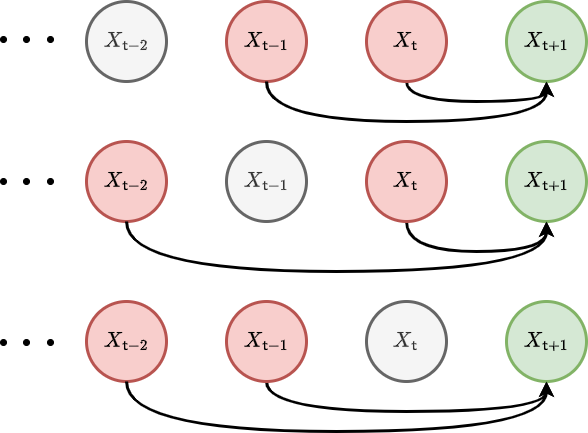
\includegraphics[width=8cm]{images/chapter-2-second-temporal-correlation.drawio.png}
\caption{Blah...}
\label{fig:second-temporal-correlation}
\end{figure} 

In a similar fashion, we can increase the expansion order of Eq.~(\ref{eq:second-order-log-expansion}) to include third-order correlations such that 
%%
\begin{align}
P_{{\sf t}+1}(X\vert z) &\rightarrow \prod_{{\sf t}'=0}^{{\sf t}}\prod_{{\sf t}''=0}^{{\sf t}'-1} P_{{\sf t}'{\sf t}''}(x',x''\vert z)P_{({\sf t}+1){\sf t}'{\sf t}''}(x\vert x',x'',z) \,,
\end{align}
%%
and, in this instance, one can show that Eq.~(\ref{eq:master-x-cont-latest-row-gen}) reduces to
%%
\begin{align}
P_{{\sf t}+1}(x\vert z) &= \frac{1}{{\sf t}}\sum_{{\sf t}'=0}^{{\sf t}}\frac{1}{{\sf t}'-1}\sum_{{\sf t}''=0}^{{\sf t}'-1}\int_{\omega_{{\sf t}'}}{\rm d}^nx'\int_{\omega_{{\sf t}''}}{\rm d}^nx'' P_{{\sf t}'{\sf t}''}(x',x''\vert z)P_{({\sf t}+1){\sf t}'{\sf t}''}(x\vert x',x'',z) \label{eq:third-order-correl} \,.
\end{align}
%%
Using $P_{{\sf t}'{\sf t}''}(x',x''\vert z) = P_{{\sf t}''}(x''\vert z) P_{{\sf t}'{\sf t}''}(x'\vert x'', z)$ one can also show that this integral is a marginalisation of this expression
%%
\begin{align}
P_{({\sf t}+1){\sf t}''}(x\vert x'', z) &= \frac{1}{{\sf t}}\sum_{{\sf t}'=0}^{{\sf t}}\int_{\omega_{{\sf t}'}}{\rm d}^nx'P_{{\sf t}'{\sf t}''}(x'\vert x'',z)P_{({\sf t}+1){\sf t}'{\sf t}''}(x\vert x',x'',z) \,,
\end{align}
%%
which describes the time evolution of the conditional probabilities.

\begin{figure}[h]
\centering
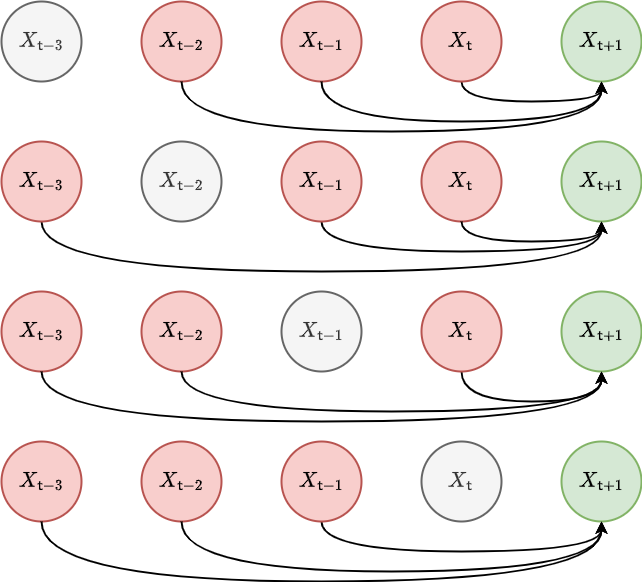
\includegraphics[width=10cm]{images/chapter-2-third-temporal-correlation.drawio.png}
\caption{Blah...}
\label{fig:third-temporal-correlation}
\end{figure} 

\textcolor{red}{
Rewrite things from here. Main goals for this chapter are:
\begin{itemize}
\item{Introduce probabilistic formalism and thinking - needs more diagrams!}
\item{Talk about mean field solutions and how some stochastic phenomena (particularly Markovian) will have averaged equations on their distribution statistics --- give some examples}
\item{Get to Gaussian processes and their kernels + discuss how they can be used to compare between separate sample datasets}
\item{Go through the learning algorithm required to set this all up but don't introduce the learnadex fully}
\end{itemize}
}

\section{\sffamily Software design}

\textcolor{red}{
\begin{itemize}
\item{Design for the Gaussian process data samples-to-simulation samples comparison algorithm in the learnadex}
\item{Also design modules for mean field sims to be compared to the stochastic sims}
\end{itemize}
}

    